%=================================================================
\documentclass[journal,article,submit,moreauthors,pdftex,10pt,a4paper]{Definitions/mdpi} 

\firstpage{1} 
\makeatletter 
\setcounter{page}{\@firstpage} 
\makeatother
\pubvolume{xx}
\issuenum{1}
\articlenumber{5}
\pubyear{2018}
\copyrightyear{2018}
%\externaleditor{Academic Editor: name}
\history{Received: date; Accepted: date; Published: date}
 
% Full title of the paper (Capitalized)
% \Title{Effect of Nanovoid on Fracture Process of Two-Phase $\gamma$($\rm TiAl$)+$\alpha_2$($\rm Ti_3Al$) Alloy}
\Title{The Effect of Void on the Cold Deformation Behaviour of $\alpha_2+\gamma$ Two Phase Ti-Al Alloy}
% Author Orchid ID: enter ID or remove command
\newcommand{\orcidauthorA}{0000-0001-8385-4439} % Add \orcidA{} behind the author's name
\newcommand{\orcidauthorB}{0000-0002-9582-6301} % Add \orcidB{} behind the author's name

% Authors, for the paper (add full first names)
\Author{Ruicheng Feng $^{1,2}$\orcidA{}, Maomao Wang $^{1}$\orcidB{}}

% Authors, for metadata in PDF
%\AuthorNames{Maomao Wang $^{1,\dagger,\ddagger}$\orcidB{}, Firstname Lastname and Firstname Lastname}

% Affiliations / Addresses (Add [1] after \address if there is only one affiliation.)
\address{%
$^{1}$ \quad School of Mechanical and Electronical Engineering, Lanzhou University of Technology, Lanzhou 730050, China; frcly@163.com (R.F.); 15620864891@163.com (M.W.)\\
% $^{2}$ \quad Key Laboratory of Digital Manufacturing Technology and Application, Ministry of Education, Lanzhou University of Technology, Lanzhou 730050, China
%*; e-mail@e-mail.com}
$^{2}$ \quad State Key Laboratory of Advanced Processing and Recycling of Non-ferrous Metals, Lanzhou University of Technology, Lanzhou 730050, China}
% Contact information of the corresponding author
\corres{Correspondence: e-mail@e-mail.com; Tel.: +x-xxx-xxx-xxxx}

% Current address and/or shared authorship
%\firstnote{Current address: Affiliation 3} 
%\secondnote{These authors contributed equally to this work.}
% The commands \thirdnote{} till \eighthnote{} are available for further notes

%\simplesumm{} % Simple summary

%\conference{} % An extended version of a conference paper

% Abstract (Do not insert blank lines, i.e. \\) 
\abstract{Fracture processes of nanocrystalline metallic materia is affected by dislocation, nanovoid and other defects. Existing studies of defect evolution in titanium-aluminium alloy cover the case that voids located in single crystals, inside grain in poly crystals and at the grain boundaries.Molecular dynamics simulation was performed to study the evolution of a spherical nanovoid in $\alpha_2$+$\gamma$ two-phase titanium-aluminium alloy under uniaxial tension. The results show that voids located at the $\alpha_2$/$\gamma$ phase boundary have significant detract to strength of Ti-Al polycrystalline.}

% Keywords
\keyword{$\alpha_2$ + $\gamma$ two phase TiAl alloy; void; molecular dynamics}

%%%%%%%%%%%%%%%%%%%%%%%%%%%%%%%%%%%%%%%%%%
\begin{document}

\section{Introduction}
TiAl alloy has been used as structural material in aviation industry because its inherent advantages such as low density and self-diffusion rates, high elastic module and high strength \cite{vu2013}. Two-phase titanium aluminum alloys with proper phase distribution and grain size exhibit better mechanical performance compared with monolithic constituents $\gamma$(TiAl) and $\gamma$($\rm Ti_3Al$) alloy \cite{Kim1995}. Brittle fracture in TiAl alloy strongly affects the safety of fracture of structure like turbo of aircraft engine and combustion generator. Deformation phenomena of TiAl alloys have been widely studied in order to overcome the problems associated with the limited ductility and damage tolerance. A great number of literature covers a wide range of parameters such as alloy composition, microstructure and deformation temperature. Much of the work has been performed on single phase $\gamma$ alloys and PST crystals[]. 
% The failure modes of materials have significant influence on the design of material properties in materials science. 
Rapture failure at the macroscopic scale can be attributed to nucleation, growth and propagation of cracks, but at the microscopic scale cracks are initially easily formed at defects in the casting process, such as voids and inclusions \cite{}. 

The initiation of crack at microscopic scale is a dynamic process, which resulting in difficulties on study of detailed mechanisms of defromation and cracking.

These defects are known to play a fundamental role in the deformation of the material. Nucleation, growth and coalescence of voids are deemed as the primary mechanism of ductile material fracture, in which void growth is particularly important. Therefore, it is necessary to study the deformation response of porous materials with the consideration of microstructure evolution.

Brittle fracture in TiAl alloy strongly affects the safety of fracture of structure like turbo of aircraft engine andcombustion generator[].Defects such as grainboundary, void and segregation plays an significant role in the process of fracture[].In order to understanding the mechanism of brittle fracture, multi-scale methods from micro to marco scale have been applied to investigate the behavior of fracture. It's necessary to carefully examine the revolution of defects and its influence on the fracture process at atomic scale.A previous study on void growth in gamma-TiAl single crystal has reveals that void with high volume fraction detracts incipient yield strength \cite{}.Molecular dynamics(MD method has been use to investigate the evolution of void in materials in nanoscale \cite{}. The fracture mechanisms in the duplex micro-structure are plasticity induced grain boundary decohesion and cleavage, while those in the lamellar microstructure are interface delamination and cracking across the lamellae \cite{}.

MD simulations has reveals that existence of voids alone may contribute to strain hardening because theyare barriers to dislocation movement \cite{Xiong2015}



\section{Molecular Dynamics Simulation }
	
\subsection{Atomic Potential}

The interaction of particle in the material is determined by interatomic potential. Many reported examples of crack propagation in metal materials were performed with embedded atomic method due to is better accuracy in metal lattice compare with F-S and L/J \cite{}. The embedded atom method (MEAM) potential developed by Zope and Mishin by \cite{} was used in the study. The simulation is submitted by MD simulations with the Large-scale Atomic/Molecular Massively Parallel Simulator (LAMMPS) open-source code \cite{}. We performed constant-pressure and constant-temperature (NPT) molecular dynamics simulation.
	
\begin{equation} \label{eq:eam} 
E_{total}= \displaystyle\sum F_i(\rho_{h,i})+\frac{1}{2}\sum_i\sum_{j(\neq1)}\phi_{ij}(R_{ij})
\end{equation}
	
where $E_{total}$ is the total energy of the system, $\rho_{h,i}$, is the host electron density at atom $i$ due to the remaining atoms of the system,$F_i(\rho)$ is the energy for embedding atom i into the background electron density $\rho$, and $\phi_{ij}(R_{ij})$ is the core-core pair repulsion between atoms $i$ and $j$ separated by the distance $R_{ij}$. It can be noted that $F_i$ only depends on the element of atom $i$ and $\phi_{ij}$ only depends on the elements of atoms $i$ and $j$. The electron density is, as stated above, approximated by the superposition of atomic densities, namely
	
%	\begin{equation} \label{eq:eam} 
%	\rho_{h,i}=\sum_{j(\neq1)} \rho_i(R_{ij})
%	\end{equation}
%	
\subsection{Model Creation of Crystalline}

\begin{figure}[ht]
	\centering
	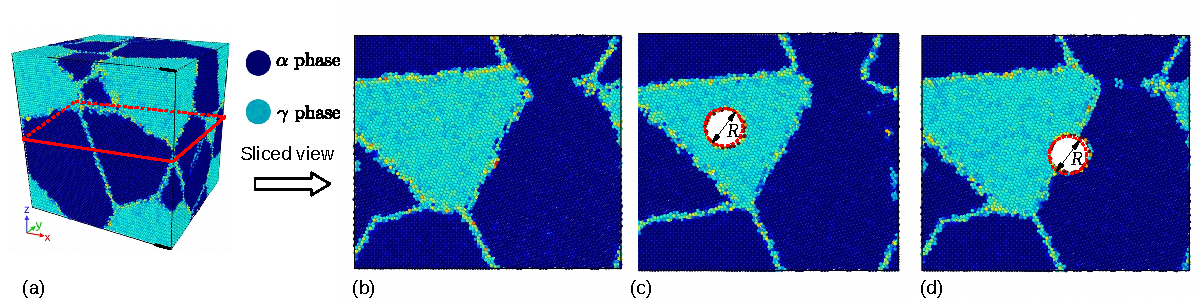
\includegraphics[width=1\linewidth]{img/models}
	\caption{Overview of model creation}
	\label{fig:model-creation}
\end{figure}

\cite{}
$\gamma $ TiAl has a fcc-centered tetragonal with an $L1_0$ structure \cite{}, and $\alpha_2 TiAl$ is hcp structure, the structure of the two initial cells are shown in Fig.\cite{}, and the constructing parameters are givin by Table.\cite{}. The simulation cells of two phase polycrystalline with an initially spherical void at different position are shown in figure \cite{}. Periodic boundary conditions (PBC)are applied along all three directions, that makes poly crystal with periodic nanovoid structures. The initial dimension of simulation cell is  $L_x = $ nm, $L_y = $ nm, $L_z = $ nm, and each model contains about 4.6 million atoms. The grain orientation and size were randomly created with Voronoi method with code ATOMSK \cite{}, and resulting in the arbitrary shape and orientation of the grains. Only one spherical void defect was placed intragranularlly or intergranularlly within each simulation model void within each simulation model. The intragranular spherical void was located in grain interior of the largest grain of the simulation model, as shown in Fig. \cite{}. The intergranular spherical void was at the center of the simulation cell, as shown in Fig. \cite{}.
	
\begin{table}[ht]
	\caption{Parameters of  nanocrystalline}
	\centering
	\begin{tabular}{l c c l}
	\toprule
	\textbf{Phase}			& \textbf{Space group}		& \textbf{Designation} 		& \textbf{Parameters} \\
	\midrule
		$\alpha_2$		& $\rm P6_3/mmc$ 	& $\rm 0_{19}$ 		& $a$ = 0.5765 \\
		&					&					& $c$ = 0.46833 \\
		$\gamma$		& $\rm tP4$ 		& $\rm L1_0$		& $a$ = 0.3997 \\
		&					&					& $c$ = 0.4062 \\			
	\bottomrule
	\end{tabular} 
	\label{tab:lattice_parameter}
\end{table} 
	
	% \begin{figure}[ht]
	% 	\centering  
	% 	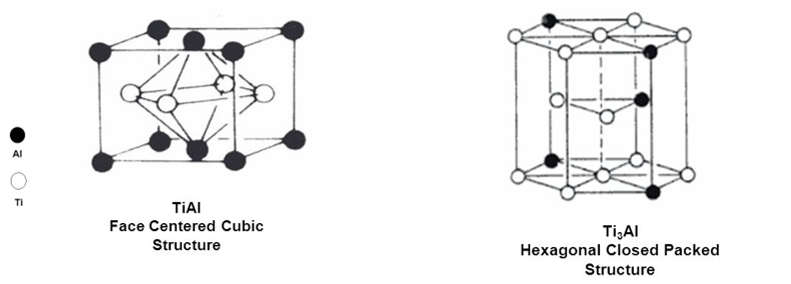
\includegraphics[width=0.7\linewidth]{img/cell}
	% 	\caption{unit cell}
	% 	\label{fig:unit_cell}
	% \end{figure}
	

\subsection{Analysis method}
The centrosymmetry parameter is defined as follow:

	\begin{equation} \label{eq:csp} 
	P = \displaystyle\sum_{i=1}^{6}|\vec{R_i}+{\vec{R}}_{i+6}|^2
	\end{equation}

where $\vec{R_i}$ and ${\vec{R}}_{i+6}$ are the vectors corresponding to the six pairs of opposite nearest neighbors in the fcc lattice. The centrosymmetry parameter(CSP) is zero for atoms in a perfect lattice. In other words, if the lattice is distorted the value of P will not be zero. Instead, the parameter will have a value within the range corresponding to a particular defect. By removing all the perfect and surface atoms within the bulk, the existence of dislocation atoms become visible.

	% \paragraph{Virial Stress}
	% The atomic stress is calculated using the virial definition :
	% $$\sigma_t(i)=-$$
	% $$\sigma_t(i)= $$
  
\section{Results and Discussion}
%	/home/alex/Documents/violet/draft/img/perfect-line.pdf
In order to examine deforamtion behaviour carefully, tensile loading was applied to the model without any types of void defect. The whole tension process was saperated into four stages: Stage-1 is typical elasttic part of the deformation, which is originated from $\epsilon = 0$ to $\epsilon = 0.092$, includeing key point 1. Stage-2 is yield stage ranging from $\epsilon = 0.092$ to $\epsilon = 0.101$, including key points 2 to 6. In stage-2, the stress decreased slightly along with the increasing of strain. Stage-3 is cracking stage and in this stage the strength of the model have beeen was detracted sharply, we can confine that the structure almost fail after the stage-3. Snapshots of atoms configuration are labeled with key points number from 1 to 10, specific list of key points numbers were shown in Table.\ref{tab:key-point}. Deformation beaviour of the $\alpha_2$ phase had $\gamma$ phase were discussed in the folling subsection respectively.

	\begin{figure}[ht]
		\centering
		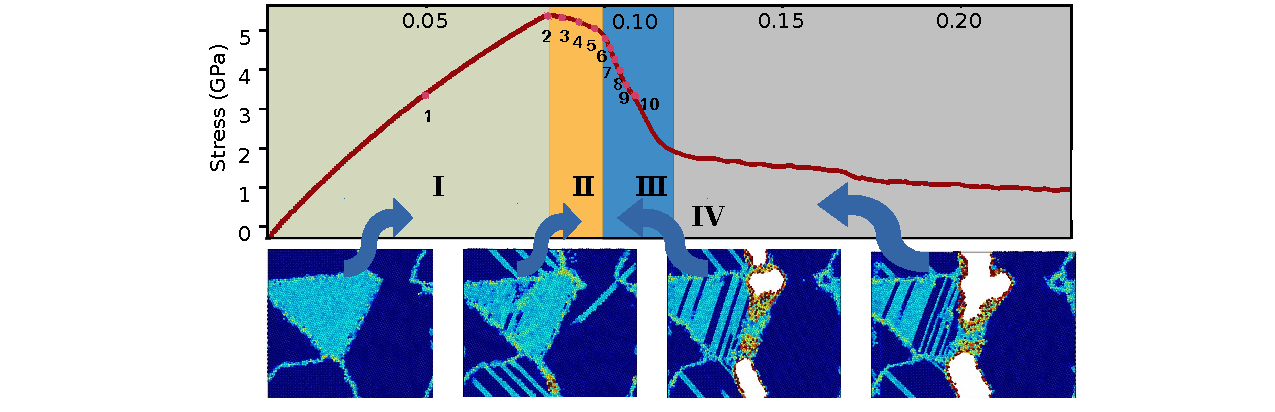
\includegraphics[width=1\linewidth]{img/perfect-line2-2}
		\caption{Deformation process of the model without void defect}
		\label{fig:deformation-pf}
	\end{figure}

	\begin{table}[ht]
		\caption{Key point during tensile process}
		\centering
		\begin{tabular}{l c c c c c c c c c c}
		\toprule
		 \textbf{Key Number} & \textbf{1} & \textbf{2} & \textbf{3} & \textbf{4} & \textbf{5} & \textbf{6} & \textbf{7} & \textbf{8} & \textbf{9} & \textbf{10}\\
		\midrule
		Time/ps	& 0 & 0.15 & 0.16 & 0.17 & 0.18 & 0.19 & 0.20 & 0.21 & 0.22 & 0.23 \\
		\midrule
		Strain	& 0 & 0.092 & 0.094 & 0.096 & 0.099 & 0.101 & 0.104 & 0.107 & 0.110 & 0.112 \\
		\bottomrule
		\end{tabular} 
		\label{tab:key-point}
	\end{table} 


\subsection{Deformation Behaviour of Two Phase Alloys without Void Defects}
However, the following discussion concentrates on deformation phenomena that rely on the elastoplastic codeformation of the $\gamma$ and $\gamma_2$ phases and on the particular point defect situation occurring in twophase alloys. Due to this effect ( $\alpha_2$ + $\gamma$ ) alloys exhibit some remarkable properties that are unlike those of either constituent.
\begin{figure}[ht]
		\centering
		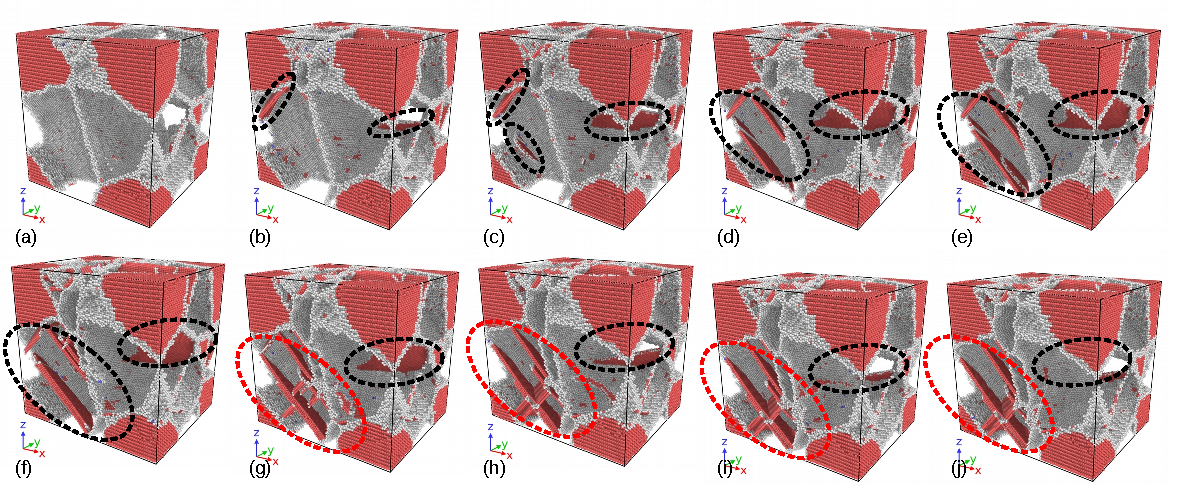
\includegraphics[width=1\linewidth]{img/def-gamma}
		\label{fig:def-gamma}
		\caption{$\gamma$ phase deformation}
\end{figure}
The configure of atoms is shown in Fig.\ref{fig:yield}, it can be seen that dislication emission initiate in $\gamma$ pahse in XXX ps, and the deformation canbe mainly confied to the majority $\gamma$ pahse. $\gamma$(TiAl) deforms by octahedral glide of ordinary dislocations with the Burgers vector b=1/2<110] and superdislocations with the Burgers vectors b=<101] and $b=1/2<11\overline{2}]$. The other potential deformation mode is mechanical twinning along $1/6<11\overline{2}]{111}$.
From Fig.\ref{fig:yield}, of the two constituents of ($\alpha_2$+$\gamma$) alloys, the $\alpha_2$ phase is more difficult to deform. A reason for the unequal strain partitioning between the $\alpha_2$ and $\gamma$ phase is certainly the strong plastic anisotropy of the $\alpha_2$ phase. TEM examinations performed on tensile  tested lamellar alloys have revealed that the limited plasticity of the $\alpha_2$ phase is mainly carried by local slip of <a>-type dislocations with the Burgers vector $b=1/3<11\overline{2}0>$ prism planes\ref{fig:yield}, which is by far the easiest slip system in $\alpha_2$ single crystals. 
	\begin{figure}[ht]
		\centering
		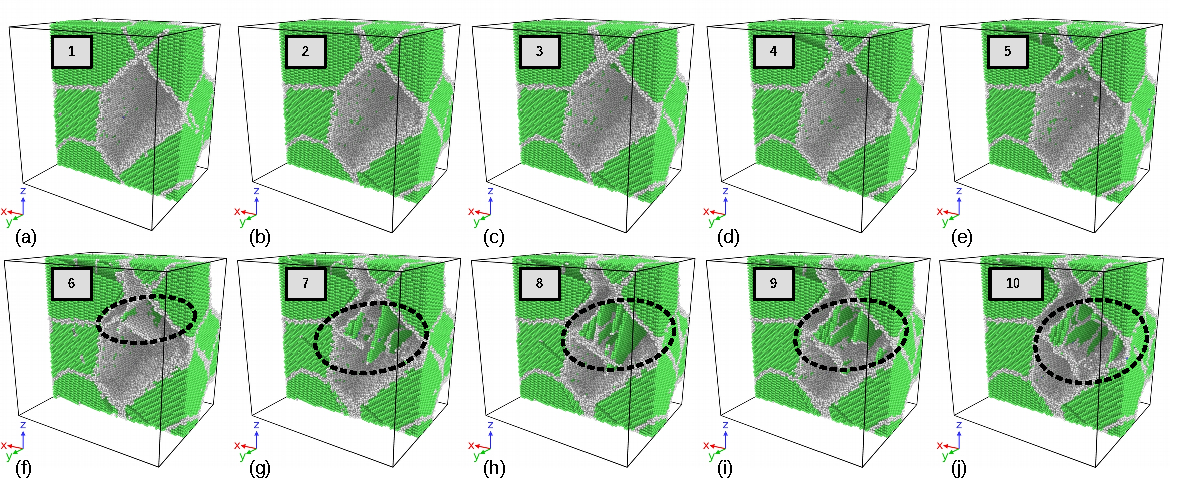
\includegraphics[width=1\linewidth]{img/def-alpha}
		\label{fig:def-alpha_2}
		\caption{$\alpha_2$ phase deformation}
	\end{figure}
Basic deformationg mechanism of $\alpha_2$ phase 

	\begin{figure}[ht]
		\centering
		\includegraphics[width=1\linewidth]{"img/disl-gamma"}
		\caption{Disloaction in $\gamma$}
		\label{fig:dis-alpha_2}
	\end{figure}

%	\begin{figure}[ht]
%		\centering
%		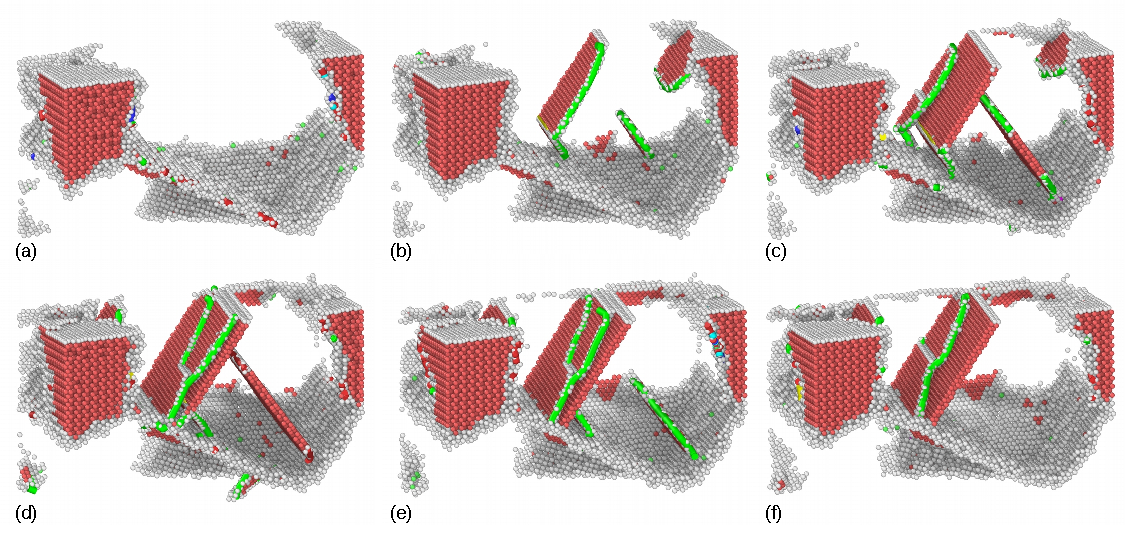
\includegraphics[width=1\linewidth]{img/disl2-gamma}
%		\label{fig:surf}
%		\caption{stress-strain curve}
%	\end{figure}
1.In many cases the orientation of slip slip is changed because the crystallographically available slip and directions are not continuous across the interface. This may significantly reduce the Schmid factor and thus impede slip transfer. At the $\gamma/\gamma$ interfaces the orientation of the slip plan could change through a relevantly large angle of about 90 degree. Reorientation of slip is always required at the $\alpha_{2}/\gamma$ interface; the smallest angle between the corresponding slip planes ${1 1 1 }_{\gamma}$ and ${ 1 0 -1 0}_{\alpha_2}$ is about 19 degree \cite{}.
	
The core of  a dislocation intersecting an interface often needs to be transformed. For example, an ordinary 1/2<110] dislocation gliding in one $\gamma$ grain has to be converted in to a <101] super dislocation with the double Burgers vector gliding in an adjacent $\gamma$ grain. At the $\alpha_2/\gamma$ interface the dislocations existing in the $D0_{19}$ structure have to be transformed into dislocations consistent with the $L1_0$structure. These core transformations are associated with a change of the dislocation line energy because the lengths of the Burgers vectors and the shear module are different.
	
Dislocations crossing semi-coherent boundaries have to intersect the misfit dislocations, a process that involves elastic interaction, jog formation and the incorporation of gliding dislocations into the mismatch structure of the interface.When the slip is forced to cross $\alpha_2$ lamella, pyramidal slip of the $\alpha_2$ phase is required, which needs an extremely high shear stress.
	
	
	%\subsection{Fracture Process with Integranular Void }
	
	%\subsection{Fracture Process with Intergranular Void }
	 
\subsection{Evolution of spherical void in the simulation with intragranular spherical voids}
The volume defects considered pertain to three-dimensional objects contained within a matrix. Three-dimensional structures composed of zero-, one- or two-dimensional defects are not considered here.
Second-phase particles, precipitated within, as a consequence of a thermal treatment, or taken up, as a consequence of a material processing route, into a matrix of the first, dominant phase, disrupt, more or less (as possibly associated with
the occurrence of incoherent or coherent interfaces; see Sect. 5.3), the long-range translation symmetry of the matrix. They may induce considerable misfit-stress fields and thus can influence material properties pronouncedly. Such stress fields surrounding the second-phase particles can be due to misfit between the volume occupied by the second-phase particle when unconstrained and the space (“hole”) put at its disposal by the matrix. Such misfit can arise due to specific volume differences induced by precipitation or by different thermal expansion or shrinkage upon heating
or cooling the specimen.
A possibly favourable effect of second-phase particles is a contribution to the enhancement of mechanical strength. Considering yielding of a material as related to glide of dislocations (Sect. 5.2.5), any mechanism obstructing dislocation glide improves the mechanical strength. In the discussion of the Frank–Read source for dislocation (-line) production (Sect. 5.2.6) it was made clear that second-phase particles can serve as obstacles for dislocation migration: the stress fields surrounding the second-phase particles can be of “antagonistic” nature and “block” propagation of the stress field of a migrating dislocation: the second-phase particle acts as “pinning point”. It was already indicated that in order that a dislocation can pass two pinning points (A and B in Fig. 5.13; see Sect. 5.2.6) a critical shear stress is needed
that depends on the distance between the obstacles (which can be second-phase particles):
\begin{equation} \label{eq:orowan} 
\tau_0 = Gb/d
\end{equation}

where d represents the distance between A and B and thus reflects the dependence of the critical shear stress $\tau_0$ on the second-phase particle density and distribution. This mechanism for hardening is designated as the Orowan process (with $\tau_0$ as the Orowan
(shear) stress ; sgitee also Sect. 11.14.4). As a result of the Orowan process, upon passage of the pinning points by a series of gliding dislocations, a system of concentric loops is formed around the second-phase particles (see Fig. 5.27). Consequently, the effective average distance between the second-phase particles has decreased to d which implies a necessary increase of the value of critical shear stress required for continuation of dislocation glide (cf. (5.10)).
A step, of the width of a burgers vector, will be generated at both sidesof a crystal along teh direction of teh burgers vector after dislocation traversing teh entire crystal, as is shown in \ref{}. A small tep will be formed at spherical void surface toward teh void interiorafter dislocation absorptionat sphericalvoid surfaces, as is shown in \ref{}. If a great number of dislocation slip along their respective systemstowards teh spherical nanovoid in all directions, and are absorbed at spherical void surfaces, the spherical nanovoid will eventually shrink from teh dash circle to

\begin{figure}[ht]
	\centering
	\includegraphics[width=1\linewidth]{"img/dis-void"}
	\caption{Dislocation around void}
	\label{fig:dis-void}
\end{figure}

\begin{figure}[ht]
	\centering
	\includegraphics[width=1\linewidth]{"img/orowan"}
	\caption{orowan}
	\label{fig:dis-void}
\end{figure}
 

	 
\subsection{The effect of void on the strength of material}

Void of R=10$\AA$ was placed at phase boundary, inside $\alpha_2$ phase grain respectively. Effect of void at different position under uniaxial tension is shown in Fig.\ref{fig:stress&strain}. The strength of materails with void in different size and at different position is shown in Fig.\ref{fig:stress&strain}. The results show that the model without void defect has best stength, while the void loacted inside $\alpha_2$ phase detracts the strength of the material most, and the void at the phase boundary have less impact on the strength.
	
The effect of siz is expectable that the greater voids detracts the strength of the materials more, however, it has been observed in the simulation that there is a critical value about 15A for voids at different position. The voids larger than 15 A have dramatic detraction to the strength of the material. Conventional definition of strength of materails with geometry substraction was applied to the model, and theroticial strength of the models was calculated by formulation \ref{eq:section}:
	
	\begin{equation} \label{eq:section} 
	\sigma^* = \sigma_0 \cdot \frac{A^*}{A_0}
	\end{equation}
	
where $\sigma_0$ is the strength of the model without void defects 5.26 Gpa, and $A_0$ is initial section area, $ A = a\times b = 36000 A^2$, $A^* $ is section area in consider of the subsection that results from the voids. Comparing with the strength determined by molecular dynamics simulation and the resuts calculated with formulation \ref{eq:section}, it can be assumed that the main factor that affects the strength of materials can be attributed to local behaciour of the materials, thus revolution of defects should be examined carefully.

	
\begin{figure}[ht]
	\centering
	\includegraphics[width=1\linewidth]{"img/fracture3"}
	\caption{Yield process of the models}
	\label{fig:yield}
\end{figure}



	\begin{figure}[ht]
		\centering
		\begin{minipage}{0.495\textwidth}
			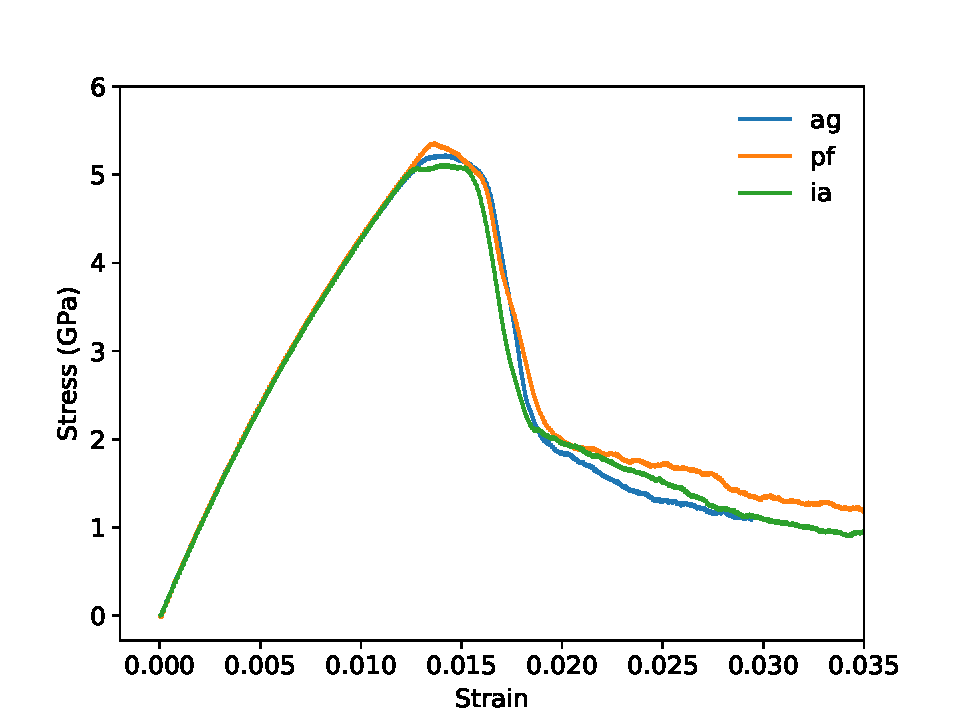
\includegraphics[width=1\linewidth]{img/allline}
			\centering
			\caption{Stress-Strain}
			\label{fig:stress&strain}
		\end{minipage}	
		\hfill
		\begin{minipage}{0.495\textwidth}		
			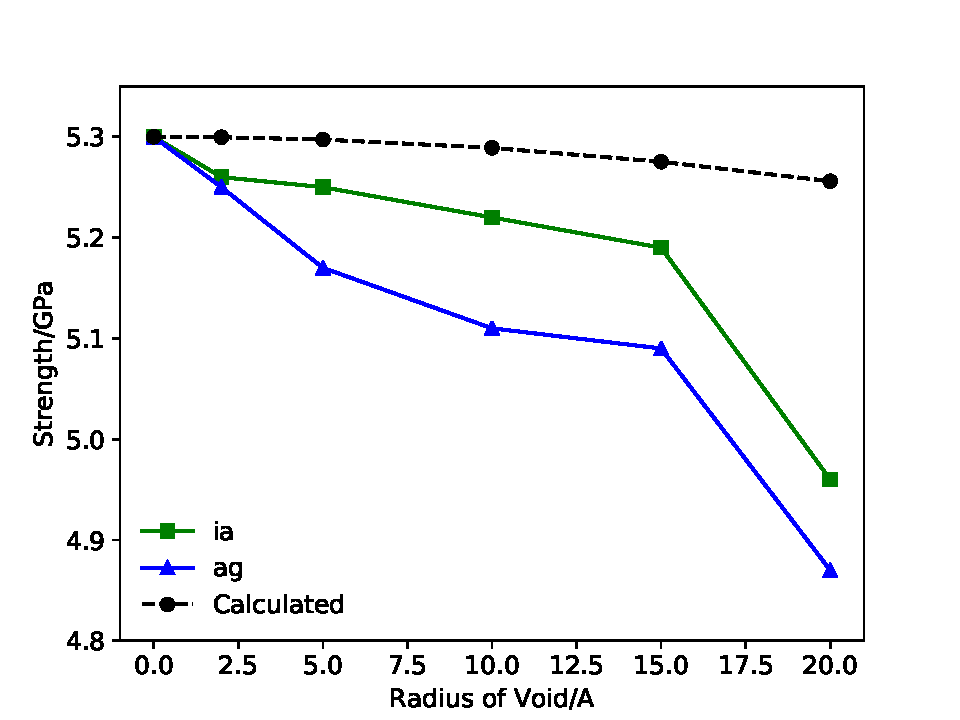
\includegraphics[width=1\linewidth]{img/effect_of_vol}
			\centering
			\caption{Strength of models}
			\label{fig:strength}
		\end{minipage}
	\end{figure}
	
	
	%\begin{figure}[ht]
	%	\centeringT
	%	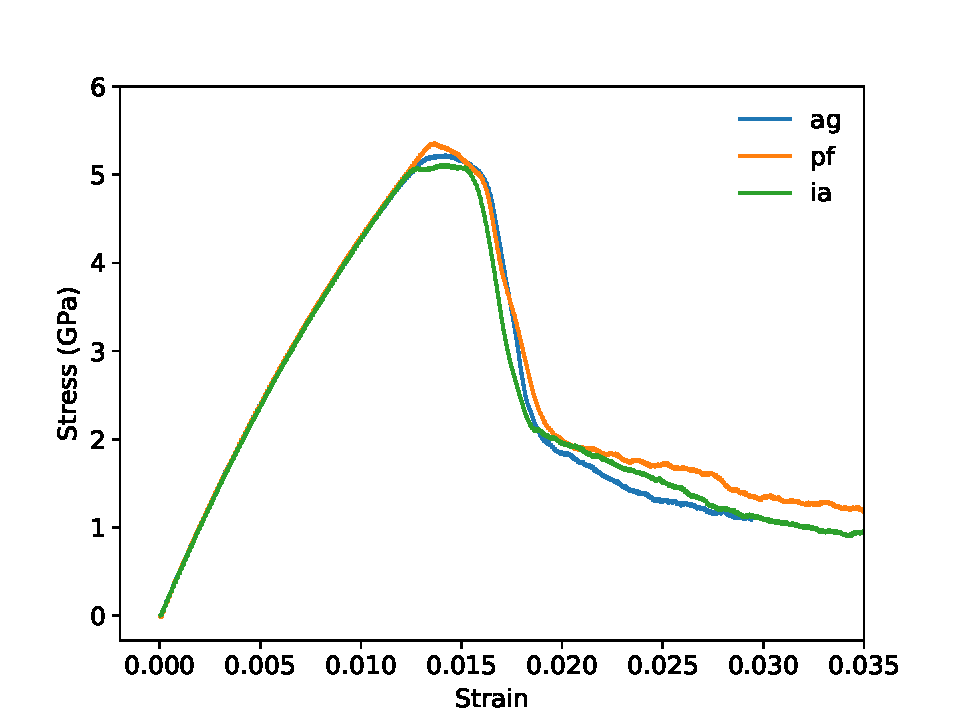
\includegraphics[width=0.7\linewidth]{img/allline}
	%	\caption{Fracture process of specimen with void in $\alpha_2$ phase}
	%	\label{ }
	%\end{figure}
	%
	
	
	
 	
	
Voids with different size: 2A, 5A, 10A, 15A were placed into the model respectively. It has been observed that  voids detracts the strengths of the material. The max stress stress of the simulation cell decreases as the volume of voids are lareger. From Fig \ref{}, there is a critical value of void radius about 15A, the void greater than 15A cause serious detraction of strength of material. 
Engineering stress is calculated
	$$ \sigma = S/A$$
The rate of decrease of loading area are smaller comparing with the detraction of strength, so it can be assumed that the yield yield behaviour and strength is much more related with local behaviour of grain boundaries and void.
	
Grain and phase boundaris are obstancles to deformation process, thus the stability of boundaries have great impact on the strength of materials. Interactive between grainboundary and void determins the fracture mode of the TiAl alloy.
	
According to Schmid's law:
	$$\tau = \sigma*m$$
where m is the Schmid factor :
	$$ m = cos(\phi)cos(\lambda)$$
	%\subsection{The influence of void on strength of TiAl alloy}
%	\begin{figure}[ht]
%		\centering
%		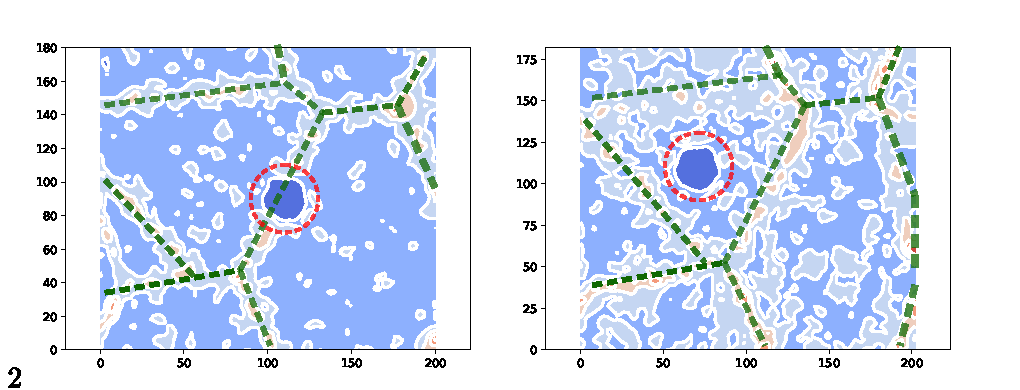
\includegraphics[width=0.7\linewidth]{img/frame2}
%		\caption{stress-$\sigma$=0}
%		\label{ }
%	\end{figure}
%	
%	\begin{figure}[ht]
%		\centering
%		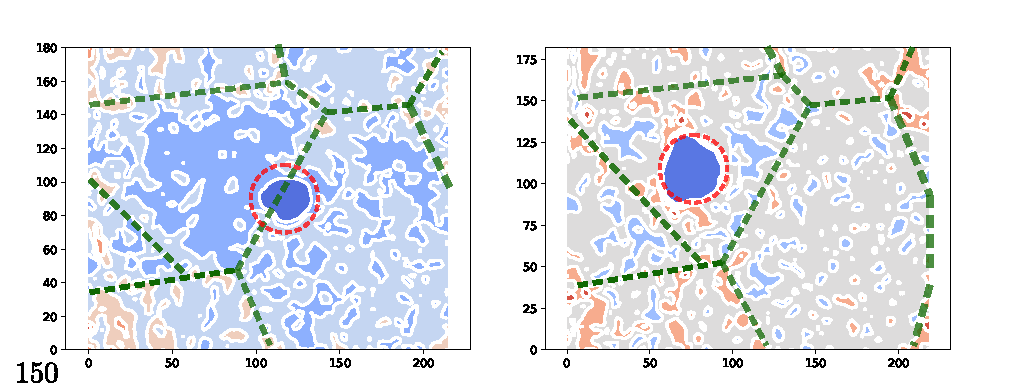
\includegraphics[width=0.7\linewidth]{img/frame150}
%		\caption{stress-$\sigma$=0.15}
%		\label{ }
%	\end{figure}
%	
%	\begin{figure}[ht]
%		\centering
%		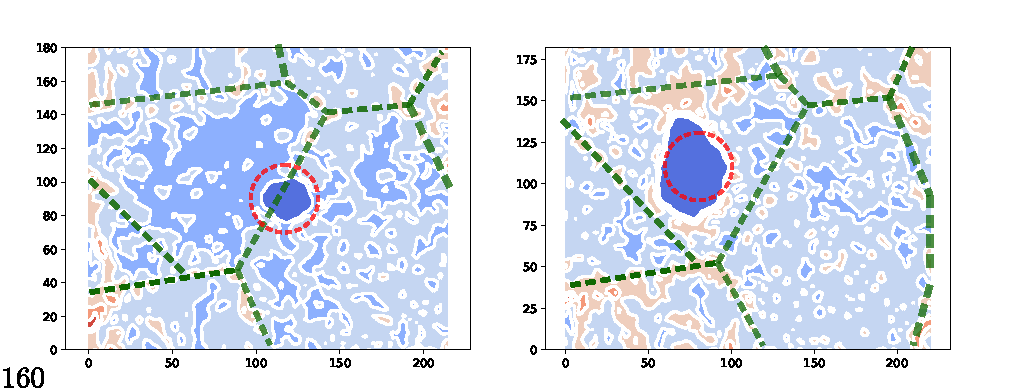
\includegraphics[width=0.7\linewidth]{img/frame160}
%		\caption{stress-$\sigma$=0.16}
%		\label{ }
%	\end{figure}
%	
%	\begin{figure}[ht]
%		\centering
%		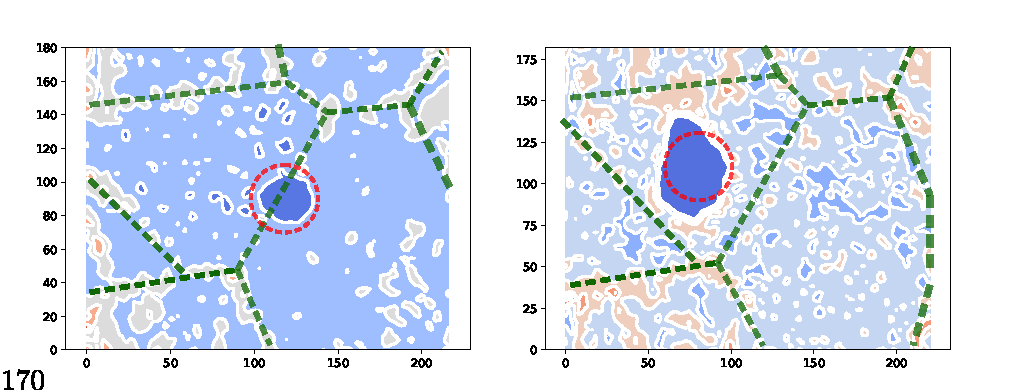
\includegraphics[width=0.7\linewidth]{img/frame170}
%		\caption{stress-$\sigma$=0.17}
%		\label{ }
%	\end{figure}
%	
%	
%	\begin{figure}[ht]
%		\centering
%		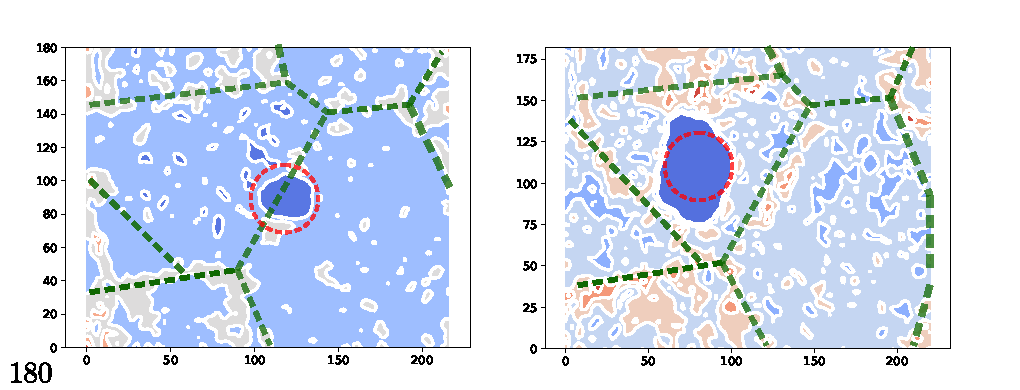
\includegraphics[width=0.7\linewidth]{img/frame180}
%		\caption{stress-$\sigma$=0.18}
%		\label{ }
%	\end{figure}
%The location of void affects strength of material. Comparing with the model with integranular void, the model with %intergranular voids is weaker. atomic stress is calculated 
%	
%	
%	
%	
%	
%	% \begin{figure}[ht]
%	% 	\centering
%	% 	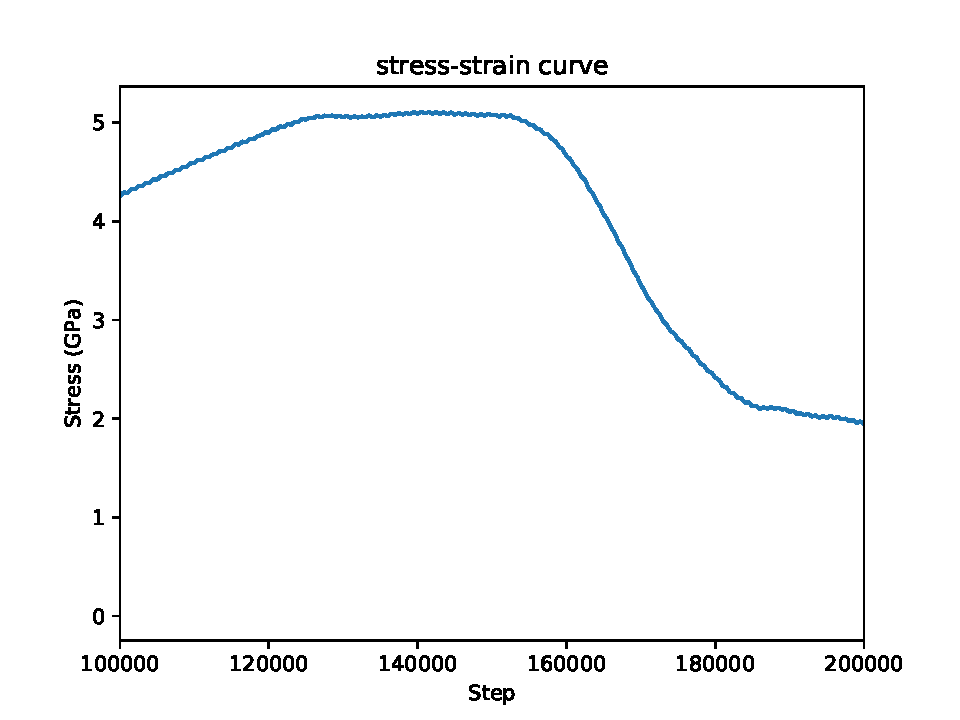
\includegraphics[width=0.7\linewidth]{img/ialine}
%	% 	\caption{stress-strain curve}
%	% 	\label{fig:ia_line}
%	% \end{figure}
%	% 
%	% \begin{figure}[ht]
%	% 	\centering
%	% 	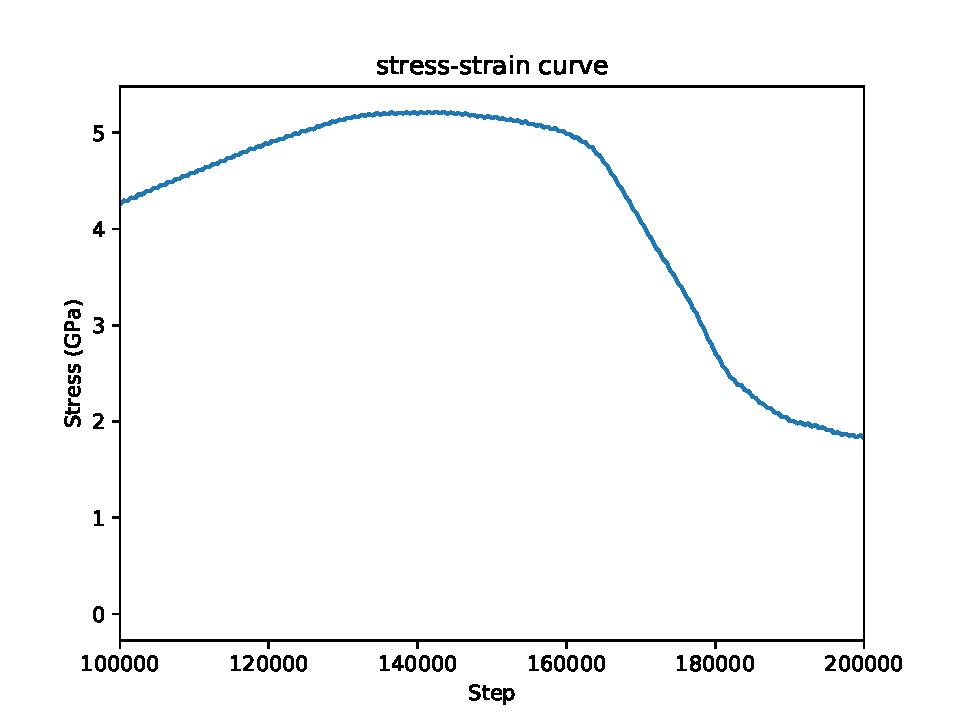
\includegraphics[width=0.7\linewidth]{img/agline}
%	% 	\caption{stress-strain curve}
%	% 	\label{fig:ag_line}
%	% \end{figure}
%	
%	
%	\begin{figure}[ht]
%		\centering
%		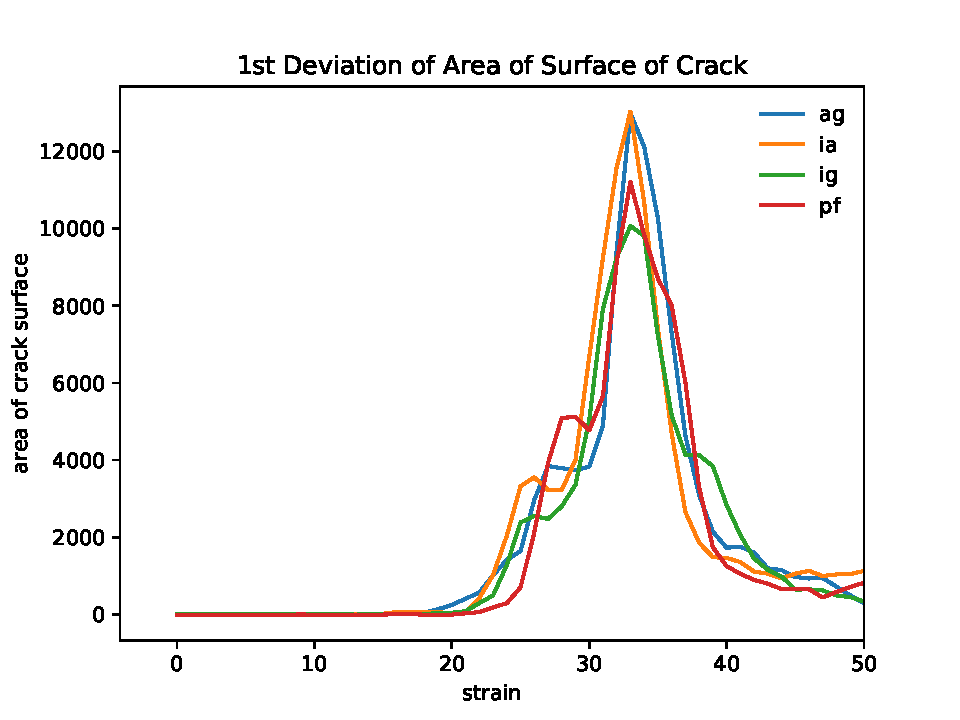
\includegraphics[width=0.7\linewidth]{img/1stdiv}
%		\label{fig:surf}
%		\caption{stress-strain curve}
%	\end{figure}
%	
%	
%	\section{Conclusion}
%	%\bibliographystyle{elsarticle-num.bst}
%	
\reftitle{References}
\bibliography{ref/VIOLET-ref.bib}
\end{document}


